%% bare_jrnl.tex
%% V1.4b
%% 2015/08/26
%% by Michael Shell
%% see http://www.michaelshell.org/
%% for current contact information.
%%
%% This is a skeleton file demonstrating the use of IEEEtran.cls
%% (requires IEEEtran.cls version 1.8b or later) with an IEEE
%% journal paper.
%%
%% Support sites:
%% http://www.michaelshell.org/tex/ieeetran/
%% http://www.ctan.org/pkg/ieeetran
%% and
%% http://www.ieee.org/

%%*************************************************************************
%% Legal Notice:
%% This code is offered as-is without any warranty either expressed or
%% implied; without even the implied warranty of MERCHANTABILITY or
%% FITNESS FOR A PARTICULAR PURPOSE! 
%% User assumes all risk.
%% In no event shall the IEEE or any contributor to this code be liable for
%% any damages or losses, including, but not limited to, incidental,
%% consequential, or any other damages, resulting from the use or misuse
%% of any information contained here.
%%
%% All comments are the opinions of their respective authors and are not
%% necessarily endorsed by the IEEE.
%%
%% This work is distributed under the LaTeX Project Public License (LPPL)
%% ( http://www.latex-project.org/ ) version 1.3, and may be freely used,
%% distributed and modified. A copy of the LPPL, version 1.3, is included
%% in the base LaTeX documentation of all distributions of LaTeX released
%% 2003/12/01 or later.
%% Retain all contribution notices and credits.
%% ** Modified files should be clearly indicated as such, including  **
%% ** renaming them and changing author support contact information. **
%%*************************************************************************


% *** Authors should verify (and, if needed, correct) their LaTeX system  ***
% *** with the testflow diagnostic prior to trusting their LaTeX platform ***
% *** with production work. The IEEE's font choices and paper sizes can   ***
% *** trigger bugs that do not appear when using other class files.       ***                          ***
% The testflow support page is at:
% http://www.michaelshell.org/tex/testflow/



\documentclass[journal]{IEEEtran}
%
% If IEEEtran.cls has not been installed into the LaTeX system files,
% manually specify the path to it like:
% \documentclass[journal]{../sty/IEEEtran}

%**** LANGUAGE PACKAGES *****
\usepackage[spanish, shorthands=off]{babel}



% Some very useful LaTeX packages include:
% (uncomment the ones you want to load)


% *** MISC UTILITY PACKAGES ***
%
%\usepackage{ifpdf}
% Heiko Oberdiek's ifpdf.sty is very useful if you need conditional
% compilation based on whether the output is pdf or dvi.
% usage:
% \ifpdf
%   % pdf code
% \else
%   % dvi code
% \fi
% The latest version of ifpdf.sty can be obtained from:
% http://www.ctan.org/pkg/ifpdf
% Also, note that IEEEtran.cls V1.7 and later provides a builtin
% \ifCLASSINFOpdf conditional that works the same way.
% When switching from latex to pdflatex and vice-versa, the compiler may
% have to be run twice to clear warning/error messages.



% *** CITATION PACKAGES ***
%
\usepackage{cite}
% cite.sty was written by Donald Arseneau
% V1.6 and later of IEEEtran pre-defines the format of the cite.sty package
% \cite{} output to follow that of the IEEE. Loading the cite package will
% result in citation numbers being automatically sorted and properly
% "compressed/ranged". e.g., [1], [9], [2], [7], [5], [6] without using
% cite.sty will become [1], [2], [5]--[7], [9] using cite.sty. cite.sty's
% \cite will automatically add leading space, if needed. Use cite.sty's
% noadjust option (cite.sty V3.8 and later) if you want to turn this off
% such as if a citation ever needs to be enclosed in parenthesis.
% cite.sty is already installed on most LaTeX systems. Be sure and use
% version 5.0 (2009-03-20) and later if using hyperref.sty.
% The latest version can be obtained at:
% http://www.ctan.org/pkg/cite
% The documentation is contained in the cite.sty file itself.


% *** GRAPHICS RELATED PACKAGES ***
%
\ifCLASSINFOpdf
 \usepackage[pdftex]{graphicx}
 \usepackage{subfigure} % subfiguras
  % declare the path(s) where your graphic files are 
 \graphicspath{ {images/} }
  % and their extensions so you won't have to specify these with
  % every instance of \includegraphics
  \DeclareGraphicsExtensions{.pdf,.jpeg,.png}
\else
  % or other class option (dvipsone, dvipdf, if not using dvips). graphicx
  % will default to the driver specified in the system graphics.cfg if no
  % driver is specified.
  % \usepackage[dvips]{graphicx}
  % declare the path(s) where your graphic files are
  % \graphicspath{{../eps/}}
  % and their extensions so you won't have to specify these with
  % every instance of \includegraphics
  % \DeclareGraphicsExtensions{.eps}
\fi
% graphicx was written by David Carlisle and Sebastian Rahtz. It is
% required if you want graphics, photos, etc. graphicx.sty is already
% installed on most LaTeX systems. The latest version and documentation
% can be obtained at: 
% http://www.ctan.org/pkg/graphicx
% Another good source of documentation is "Using Imported Graphics in
% LaTeX2e" by Keith Reckdahl which can be found at:
% http://www.ctan.org/pkg/epslatex
%
% latex, and pdflatex in dvi mode, support graphics in encapsulated
% postscript (.eps) format. pdflatex in pdf mode supports graphics
% in .pdf, .jpeg, .png and .mps (metapost) formats. Users should ensure
% that all non-photo figures use a vector format (.eps, .pdf, .mps) and
% not a bitmapped formats (.jpeg, .png). The IEEE frowns on bitmapped formats
% which can result in "jaggedy"/blurry rendering of lines and letters as
% well as large increases in file sizes.
%
% You can find documentation about the pdfTeX application at:
% http://www.tug.org/applications/pdftex





% *** MATH PACKAGES ***
%
\usepackage{amsmath}
% A popular package from the American Mathematical Society that provides
% many useful and powerful commands for dealing with mathematics.
%
% Note that the amsmath package sets \interdisplaylinepenalty to 10000
% thus preventing page breaks from occurring within multiline equations. Use:
%\interdisplaylinepenalty=2500
% after loading amsmath to restore such page breaks as IEEEtran.cls normally
% does. amsmath.sty is already installed on most LaTeX systems. The latest
% version and documentation can be obtained at:
% http://www.ctan.org/pkg/amsmath





% *** SPECIALIZED LIST PACKAGES ***
%
\usepackage{algorithmic}
% algorithmic.sty was written by Peter Williams and Rogerio Brito.
% This package provides an algorithmic environment fo describing algorithms.
% You can use the algorithmic environment in-text or within a figure
% environment to provide for a floating algorithm. Do NOT use the algorithm
% floating environment provided by algorithm.sty (by the same authors) or
% algorithm2e.sty (by Christophe Fiorio) as the IEEE does not use dedicated
% algorithm float types and packages that provide these will not provide
% correct IEEE style captions. The latest version and documentation of
% algorithmic.sty can be obtained at:
% http://www.ctan.org/pkg/algorithms
% Also of interest may be the (relatively newer and more customizable)
% algorithmicx.sty package by Szasz Janos:
% http://www.ctan.org/pkg/algorithmicx



\usepackage{xspace} 

% *** ALIGNMENT PACKAGES ***
%
\usepackage{array}
% Frank Mittelbach's and David Carlisle's array.sty patches and improves
% the standard LaTeX2e array and tabular environments to provide better
% appearance and additional user controls. As the default LaTeX2e table
% generation code is lacking to the point of almost being broken with
% respect to the quality of the end results, all users are strongly
% advised to use an enhanced (at the very least that provided by array.sty)
% set of table tools. array.sty is already installed on most systems. The
% latest version and documentation can be obtained at:
% http://www.ctan.org/pkg/array


% IEEEtran contains the IEEEeqnarray family of commands that can be used to
% generate multiline equations as well as matrices, tables, etc., of high
% quality.




% *** SUBFIGURE PACKAGES ***
%\ifCLASSOPTIONcompsoc
%  \usepackage[caption=false,font=normalsize,labelfont=sf,textfont=sf]{subfig}
%\else
%  \usepackage[caption=false,font=footnotesize]{subfig}
%\fi
% subfig.sty, written by Steven Douglas Cochran, is the modern replacement
% for subfigure.sty, the latter of which is no longer maintained and is
% incompatible with some LaTeX packages including fixltx2e. However,
% subfig.sty requires and automatically loads Axel Sommerfeldt's caption.sty
% which will override IEEEtran.cls' handling of captions and this will result
% in non-IEEE style figure/table captions. To prevent this problem, be sure
% and invoke subfig.sty's "caption=false" package option (available since
% subfig.sty version 1.3, 2005/06/28) as this is will preserve IEEEtran.cls
% handling of captions.
% Note that the Computer Society format requires a larger sans serif font
% than the serif footnote size font used in traditional IEEE formatting
% and thus the need to invoke different subfig.sty package options depending
% on whether compsoc mode has been enabled.
%
% The latest version and documentation of subfig.sty can be obtained at:
% http://www.ctan.org/pkg/subfig




% *** FLOAT PACKAGES ***
%
%\usepackage{fixltx2e}
% fixltx2e, the successor to the earlier fix2col.sty, was written by
% Frank Mittelbach and David Carlisle. This package corrects a few problems
% in the LaTeX2e kernel, the most notable of which is that in current
% LaTeX2e releases, the ordering of single and double column floats is not
% guaranteed to be preserved. Thus, an unpatched LaTeX2e can allow a
% single column figure to be placed prior to an earlier double column
% figure.
% Be aware that LaTeX2e kernels dated 2015 and later have fixltx2e.sty's
% corrections already built into the system in which case a warning will
% be issued if an attempt is made to load fixltx2e.sty as it is no longer
% needed.
% The latest version and documentation can be found at:
% http://www.ctan.org/pkg/fixltx2e


%\usepackage{stfloats}
% stfloats.sty was written by Sigitas Tolusis. This package gives LaTeX2e
% the ability to do double column floats at the bottom of the page as well
% as the top. (e.g., "\begin{figure*}[!b]" is not normally possible in
% LaTeX2e). It also provides a command:
%\fnbelowfloat
% to enable the placement of footnotes below bottom floats (the standard
% LaTeX2e kernel puts them above bottom floats). This is an invasive package
% which rewrites many portions of the LaTeX2e float routines. It may not work
% with other packages that modify the LaTeX2e float routines. The latest
% version and documentation can be obtained at:
% http://www.ctan.org/pkg/stfloats
% Do not use the stfloats baselinefloat ability as the IEEE does not allow
% \baselineskip to stretch. Authors submitting work to the IEEE should note
% that the IEEE rarely uses double column equations and that authors should try
% to avoid such use. Do not be tempted to use the cuted.sty or midfloat.sty
% packages (also by Sigitas Tolusis) as the IEEE does not format its papers in
% such ways.
% Do not attempt to use stfloats with fixltx2e as they are incompatible.
% Instead, use Morten Hogholm'a dblfloatfix which combines the features
% of both fixltx2e and stfloats:
%
% \usepackage{dblfloatfix}
% The latest version can be found at:
% http://www.ctan.org/pkg/dblfloatfix




%\ifCLASSOPTIONcaptionsoff
%  \usepackage[nomarkers]{endfloat}
% \let\MYoriglatexcaption\caption
% \renewcommand{\caption}[2][\relax]{\MYoriglatexcaption[#2]{#2}}
%\fi
% endfloat.sty was written by James Darrell McCauley, Jeff Goldberg and 
% Axel Sommerfeldt. This package may be useful when used in conjunction with 
% IEEEtran.cls'  captionsoff option. Some IEEE journals/societies require that
% submissions have lists of figures/tables at the end of the paper and that
% figures/tables without any captions are placed on a page by themselves at
% the end of the document. If needed, the draftcls IEEEtran class option or
% \CLASSINPUTbaselinestretch interface can be used to increase the line
% spacing as well. Be sure and use the nomarkers option of endfloat to
% prevent endfloat from "marking" where the figures would have been placed
% in the text. The two hack lines of code above are a slight modification of
% that suggested by in the endfloat docs (section 8.4.1) to ensure that
% the full captions always appear in the list of figures/tables - even if
% the user used the short optional argument of \caption[]{}.
% IEEE papers do not typically make use of \caption[]'s optional argument,
% so this should not be an issue. A similar trick can be used to disable
% captions of packages such as subfig.sty that lack options to turn off
% the subcaptions:
% For subfig.sty:
% \let\MYorigsubfloat\subfloat
% \renewcommand{\subfloat}[2][\relax]{\MYorigsubfloat[]{#2}}
% However, the above trick will not work if both optional arguments of
% the \subfloat command are used. Furthermore, there needs to be a
% description of each subfigure *somewhere* and endfloat does not add
% subfigure captions to its list of figures. Thus, the best approach is to
% avoid the use of subfigure captions (many IEEE journals avoid them anyway)
% and instead reference/explain all the subfigures within the main caption.
% The latest version of endfloat.sty and its documentation can obtained at:
% http://www.ctan.org/pkg/endfloat
%
% The IEEEtran \ifCLASSOPTIONcaptionsoff conditional can also be used
% later in the document, say, to conditionally put the References on a 
% page by themselves.




% *** PDF, URL AND HYPERLINK PACKAGES ***
%
%\usepackage{url}
% url.sty was written by Donald Arseneau. It provides better support for
% handling and breaking URLs. url.sty is already installed on most LaTeX
% systems. The latest version and documentation can be obtained at:
% http://www.ctan.org/pkg/url
% Basically, \url{my_url_here}.


\usepackage{authblk}

% *** Do not adjust lengths that control margins, column widths, etc. ***
% *** Do not use packages that alter fonts (such as pslatex).         ***
% There should be no need to do such things with IEEEtran.cls V1.6 and later.
% (Unless specifically asked to do so by the journal or conference you plan
% to submit to, of course. )


% correct bad hyphenation here
\hyphenation{op-tical net-works semi-conduc-tor}

% Paquete para saltos del inea
\usepackage[utf8]{inputenc}


% Paquete para utilizar colores
\usepackage{color}



\begin{document}
%
% paper title
% Titles are generally capitalized except for words such as a, an, and, as,
% at, but, by, for, in, nor, of, on, or, the, to and up, which are usually
% not capitalized unless they are the first or last word of the title.
% Linebreaks \\ can be used within to get better formatting as desired.
% Do not put math or special symbols in the title.
\title{ 10 Experimentos Científicos más Bellos de la Historia }
%
%
% author names and IEEE memberships
% note positions of commas and nonbreaking spaces ( ~ ) LaTeX will not break
% a structure at a ~ so this keeps an author's name from being broken across
% two lines.
% use \thanks{} to gain access to the first footnote area
% a separate \thanks must be used for each paragraph as LaTeX2e's \thanks
% was not built to handle multiple paragraphs
%

\author{Manuel Figueroa,\IEEEmembership{ Estudiante, ITCR,}
        Esteban Leandro,\IEEEmembership{ Estudiante, ITCR}}% <-this % stops a space
\affil[]{\textit{MC-7201 Introducción a la Investigación}}
\affil[]{\textit{Instituto Tecnológico de Costa Rica}}
\affil[]{\textit{\{mfigueroacr, elc790\}@gmail.com}}

% note the % following the last \IEEEmembership and also \thanks - 
% these prevent an unwanted space from occurring between the last author name
% and the end of the author line. i.e., if you had this:
% 
% \author{....lastname \thanks{...} \thanks{...} }
%                     ^------------^------------^----Do not want these spaces!
%
% a space would be appended to the last name and could cause every name on that
% line to be shifted left slightly. This is one of those "LaTeX things". For
% instance, "\textbf{A} \textbf{B}" will typeset as "A B" not "AB". To get
% "AB" then you have to do: "\textbf{A}\textbf{B}"
% \thanks is no different in this regard, so shield the last } of each \thanks
% that ends a line with a % and do not let a space in before the next \thanks.
% Spaces after \IEEEmembership other than the last one are OK (and needed) as
% you are supposed to have spaces between the names. For what it is worth,
% this is a minor point as most people would not even notice if the said evil
% space somehow managed to creep in.



% The paper headers
\markboth{ININ Tarea Corta 2: Experimentos más bellos de la historia , Octubre 2019}%
{Shell \MakeLowercase{\textit{et al.}}: Experimentos más bellos de la historia}
% The only time the second header will appear is for the odd numbered pages
% after the title page when using the twoside option.
% 
% *** Note that you probably will NOT want to include the author's ***
% *** name in the headers of peer review papers.                   ***
% You can use \ifCLASSOPTIONpeerreview for conditional compilation here if
% you desire.




% If you want to put a publisher's ID mark on the page you can do it like
% this:
%\IEEEpubid{0000--0000/00\$00.00~\copyright~2015 IEEE}
% Remember, if you use this you must call \IEEEpubidadjcol in the second
% column for its text to clear the IEEEpubid mark.



% use for special paper notices
%\IEEEspecialpapernotice{(Invited Paper)}




% make the title area
\maketitle

% As a general rule, do not put math, special symbols or citations
% in the abstract or keywords.
% \begin{abstract}

% \end{abstract}

% Note that keywords are not normally used for peerreview papers.
\begin{IEEEkeywords}
\LaTeX\xspace , Introducción a la investigación, Tarea Corta, Experimentos, Historia.
\end{IEEEkeywords}






% For peer review papers, you can put extra information on the cover
% page as needed:
% \ifCLASSOPTIONpeerreview
% \begin{center} \bfseries EDICS Category: 3-BBND \end{center}
% \fi
%
% For peerreview papers, this IEEEtran command inserts a page break and
% creates the second title. It will be ignored for other modes.
\IEEEpeerreviewmaketitle



\section{Erátostenes y la circunferencia de la tierra}
%*******************************Usos acádemicos extension e importancia*******************************%
\subsection{Contexto Histórico}
Eratóstenes fue un académico de la antigua Grecia (276 a.C - 195 a.C) conocido por realizar la primera medición conocida
de la Tierra. Eratóstenes parte de la suposición griega de que la tierra es esférica,
y que en comparación con otros cuerpos celestes,
esta era diminuta. Esto se explica en la obra \emph{Acerca del clelo},
de Aristóteles y escrita un siglo antes de Eratóstenes.
Entre los argumentos lógicos de la obra se mencionan entre otros hechos que los viajeros ven 
estrellas distintas si viajan al norte o al sur y que algunas estrellas visibles en lugares como Egipto o Chipre no son visibles en lugares más 
septentrionales.
Eratóstenes nació al norte de África, y se educó en Atenas, fue un pensador influyente en muchas áreas y escribió \emph{Geographica}, una obra de 
geografía conocida por ser la primera en utilizar el sistema de parelos y meridianos conocido en la actualidad.

\subsection{El experimento}
Eratóstenes buscaba obtener una medición más precisa y verificar o desmentir estimaciones anteriores del tamaño real de la Tierra.
Aristóteles calculaba este tamaño en 400.000 estadios que es aproximadamente unos 64.000 kilómetros, algo lejos del valor real del diámetro de la Tierra (40.000 Km)
Eratóstenes asumió que si la tierra era de hecho un cuerpo pequeño y esférico, entonces otros cuerpos como el Sol deberían de encontrarse muy lejos  de manera que sus rayos
deberían ser prácticamente paralelos en todos los puntos de la Tierra.

Utilizando este hecho como base de su experimento y 
conociendo por relatos que en la ciudad de Siena (Asuán, Egipto)
durante el solsticio de verano el sol del mediodía se ubicaba justo por encima de la cabeza. De este modo
no se proyectaba ninguna sombra en un objeto vertical.

Al mismo tiempo en Alejandría, ciudad ubicada al norte de Siena, se conocía que nunca se podía observar al sol 
directamente sobre la cabeza, razón por la cuál los objetos verticales siempre proyectaban una sombra.

Este hecho, sirvió a Eratóstenes para realizar los cálculos de medición de la circunferencia de la tierra con gran precisión.
La simplicidad del experimento permite determinar dimensiones cósmicas midiendo unicamente la longitud de la sombra proyctada por 
un reloj solar en Alejandría, mientras que en Siena ocurría el solsticio y no se proyectaba sombra.

De manera similar al siguiente gráfico:
\begin{center}
  \begin{figure}[h!]
  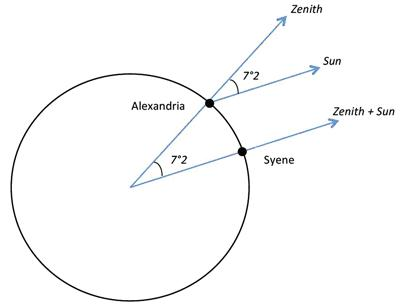
\includegraphics[width=60mm]{Eratostenes.jpg}
  \caption{Cálculo realizado por Eratóstenes.}
  \end{figure}
\end{center}

Deacuerdo a la geometría Euclideana, los ángulos interiores
de una línea que interseca dos líneas paralelas son iguales, por lo tanto el ángulo formado por el Zenith y el Sol, es igual al formado
por los radios desde el centro de la tierra a Siena y Alejandría.

Esto le sirvió para determinar la fracción de la circunferencia representada por la distancia ya conocida entre Siena y Alejandría que había sido 
determinada por los topográfos reales del gobierno Egipcio, con esto logró determinar el tamaño de la circunferencia 
de la Tierra en unos 252 000 estadios, lo que es aproximadamente 40.200 Km una cifra bastante cercana a la aceptada en la actualidad de 40.075Km \cite{crease_2014}

\section{Hershey - Chase: Función genética del ADN}
\subsection{Contexto Histórico}

A principios del siglo XX se aceptaba que el material genético de las células
era formado por proteínas. Esto principalmente a que se conocía que la estructura 
del ADN, por las investigaciones de Phoebus Levene en 1933, consistía de cuatro elementos llamados
nucleótidos.
Debido a esta limitación en la cantidad de bloques que formaban las estructuras de ADN se consideraba
imposible que este sirviese como mecánismo para transferir información genética, como el color de piel, ojos, entre otros.
Las proteínas, elementos también presentes en las células ofrecían un mayor factor de diversidad y podían combinarse de muchas más maneras. Por esta
razón se creía que eran estas las encargadas de transmitir las características en cada generación.

En 1935, Oswald Avery realizó una serie de experimentos que mostraron que el ADN facilitaba un fénomeno genético en las bacterias, pudiendo demostrar que el factor de herencia 
que causaba transformaciones en las bacterias contenía ADN. Sin embargo, no se pudo descartar que otros componentes sin ADN estuviesen involucrados en dicha transformación.
Por esta razón, muchos científicos seguían considerando a las proteínas como las encargadas de transmitir la herencia genética de las células.

\subsection{El experimento}
En 1951, los científicos Alfred Hershey y Martha Chase iniciaron una serie de experimentos con el objetivo de desacreditar
las afirmaciones de Avery. En sus experimentos se analizó como los bacteriófagos infectaban las bacterias.
Descubrieron que cuando un fago infecta a una bacteria, inicialmente se pega al exterior de la bacteria y despues inserta parte de su contenido 
al interior de la bacteria, lo que le permite replicarse dentro de la misma y generar nuevos bacteriófagos que invadan a las células cercanas.

La técnica utilizada por Hershey y Chase consistía en usar etiquetas de isótopos radiactivos.
Los elementos químicos pueden existir en diferentes formas estructurales denominadas isótopos, que pueden 
tener diferentes niveles de radiactividad que pueden ser detectados por los científicos y de esta manera determinar si las partes etiquetadas fueron transmitidas de los fagos a las bacterias.

Etiquetando la parte de proteínas  del bacteriófago con isótopos de azufre y el ADN con fósforo radiactivo, y utilizando una licuadora común, descubrieron que las proteínas permitían al fago
pegarse a la membrana superficial de la bactería y lo que se inyectaba dentro del interior de la bactería era de hecho el ADN del bacteriófago, y por lo tanto lo
que permitía la replicación de nuevos bacteriófagos en el interior de la bacteria infectada.

Los resultados de medir la mezcla descubrieron que al licuar las bacterias infectadas se removía hasta el 80\% de las proteínas marcas y solamente cerca del 40\% del ADN marcado
indicando que el material restante se había incorporado al interior de las céulas.

Con este experimento demostraron que Avery estaba en lo correcto y que el componente de la herencia genética
es en realidad el ADN y no las proteínas como se creía.

Por esta serie de experimentos Hershey recibe el premio Nobel en 1969.
\begin{center}
  \begin{figure}[h!]
  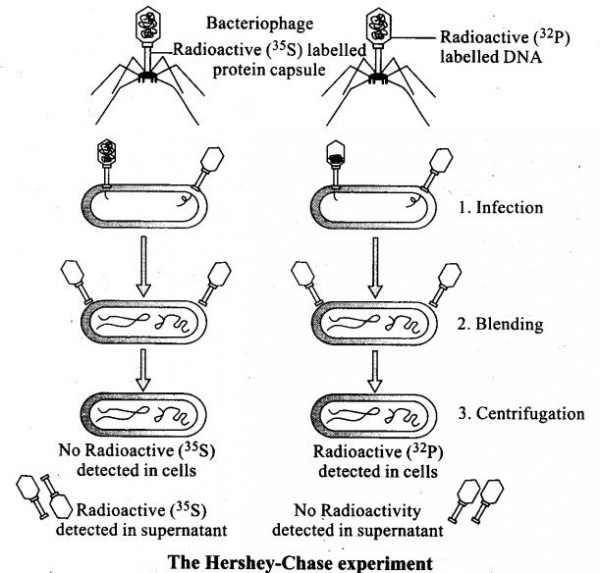
\includegraphics[width=60mm]{hershey.jpg}
  \caption{Experimento Hershey-Chase .}
  \end{figure}
\end{center}
%************************Manejo de Texto **************************************/
\section{Manejo de Texto}
\subsection{Manejo de párrafos}
\LaTeX\xspace  permite un manejo fluido y natural de los párrafos, por lo que simplemente basta con dejar una línea en blanco entre el texto y automáticamente se va a crear un nuevo párrafo en el documento.

\begin{center}
\begin{verbatim}
  
    Lorem ipsum dolor adipiscing elit, 
    mattis pharetra curabitur.
    
    Dapibus egestas blandit dictumst.
\end{verbatim}
\end{center}


El ejemplo anterior produce el siguiente texto con la clara división entre párrafos.
\begin{center}
  Lorem ipsum dolor adipiscing elit, 
  mattis pharetra curabitur.
  
  Dapibus egestas blandit dictumst.
\end{center}
Otra manera de generar párrafos en \LaTeX\xspace  es hacer uso del comando \textbackslash{}par.
Simplemente se coloca en el texto donde se quiere generar un nuevo párrafo.
\subsubsection{Alineación de párrafos}
Existen comandos útiles para definir la alineación del texto de un párrafo:
\begin{itemize}
  \item \textbackslash{}center: Para alinear al centro.
  \item \textbackslash{}flushleft: Alinea a la izquierda.
  \item \textbackslash{}flushright: Alinea a la derecha.
\end{itemize}

\subsubsection{Identación}

Por defecto \LaTeX\xspace  no hace identación del primer párrafo de una sección o capítulo.
La identación de los demás párrafos está definida por el valor definido usando \textbackslash{}parindent
Por ejemplo:
\begin{center}
  \begin{verbatim}
  \documentclass{article} 
  \setlength{\parindent}{4em} 
  \begin{document}
    ...
  \end{document}
  \end{verbatim}
\end{center}

\subsubsection{Espaciado entre líneas}
Para definir un valor diferente al por defecto para el espaciado entre las líneas de un párrafo se utiliza el comando:
\begin{center}
  \begin{verbatim}
    \renewcommand{\baselinestretch}{1.5}
  \end{verbatim}  
\end{center}

\subsubsection{Efectos de letra}
\LaTeX\xspace  permite aplicar efectos al texto para enfatizar conceptos y palabras clave que deseamos resaltar. El emplear estos efectos de manera apropiada permite que los lectores encuentren nuestro artículo más fácil de comprender.
Para aplicar texto en cursiva empleamos el comando \textbackslash{}\textbf{\textit{textit}}\{Texto en cursiva\}, lo que produce:
\textit{Texto en cursiva}.

Para subrayar el texto el comando empleado es  \textbackslash{}\textbf{\textit{underline}}\{Texto subrayado\}, 
lo que se puede ver como: \underline{Texto subrayado}.

Para poder enfatizar utilizando el efecto de negrita en las letras de una palabra o frase se emplea el comando \textbackslash{}\textbf{textbf}\{Texto en negrita\}.

Otro mecanismo de énfasis para el texto es el comando  \textbackslash{}\textbf{\textit{emph}}\{Texto enfatizado\}, este comando permite entre otras cosas resaltar el texto sin importar el 
formato original del párrafo por lo que si se encontraba en un texto en cursiva provoca el efecto contrario para mantener el énfasis de la frase deseada. Por ejemplo:

\textit{Este texto está en cursiva y \emph{este otro está enfatizado}}.

\LaTeX\xspace  también permite cambiar el tamaño del texto para lo cual tenemos los siguientes comandos:

\begin{center}
  \begin{tabular}[t]{|m{3cm}|m{3cm}|}
    \hline
    \textbackslash{}tiny\{A\} & \tiny{A} \\ \hline
    \textbackslash{}scriptsize\{A\} & \scriptsize{A} \\ \hline
    \textbackslash{}small\{A\} & \small{A} \\ \hline
    \textbackslash{}normalsize\{A\} & \normalsize{A} \\ \hline
    \textbackslash{}large\{A\} & \large{A} \\ \hline
    \textbackslash{}huge\{A\} & \huge{A} \\ \hline
  \end{tabular}  
\end{center}

\subsubsection{Manejo de tildes}
Los acentos suelen generar problemas cuando se trabaja colaborativamente en un documento, debido a que distintos usuarios
emplean sistemas operativos distintos, con configuraciones locales distintas y diferentes codificaciones de texto. Es por esto  que para tildar 
letras y aplicar acentos se recomienda utilizar el comando \textbackslash{}'A para producir \'A.

\subsubsection{Títulos}

Para establecer el título del documento se usa el comando \emph{\textbackslash{}title}\{Titulo del Documento\}.
También existen comandos para los títulos de secciones intermedias del documento como \emph{\textbackslash{}chapter} para 
iniciar un nuevo capítulo, o el comando \emph{\textbackslash{}section} para establecer una nueva sección.

\subsubsection{Manejo de referencias}

\LaTeX\xspace  ofrece un soporte completo para el manejo de referencias
y citas en el texto, ya que son una parte fundamental en la producción de textos científicos.
Para el manejo de referencias se puede utilizar el comando \emph{\textbackslash{}begin\{thebibliography\}} 
\begin{center}
\small{
\begin{verbatim}
  \begin{thebibliography}{1}

    \bibitem{IEEEhowto:kopka}
    H.~Kopka and P.~W. Daly, 
    \emph{A Guide to \LaTeX\xspace },
    3rd~ed.\hskip 1em plus 
    0.5em minus 0.4em\relax Harlow,
    England: Addison-Wesley, 1999.
    
    \end{thebibliography}
\end{verbatim}}
\end{center}

Otra manera de crear referencias en un documento es utilizando la herramienta BibTeX que permite crear un 
archivo externo con todas las referencias del documento y simplemente agregar las citas necesarias cuando estas sean requeridas.

Para realizar una cita bibliográfica se emplea el comando \emph{\textbackslash{}cite} con la etiqueta que identifica de manera única a la entrada
de las referencias a la que queremos citar.

\subsubsection{Marcas de agua}
Existe un paquete para \LaTeX\xspace  que permite la creación de marcas de agua en el documento \cite{callegar_2015}.
Al usar dicho paquete tenemos las opciones:
\begin{itemize}
\item \emph{\textbackslash{}SetWatermarkText\{Texto\}:} Permite definir el texto de la marca de agua.   
\item \emph{\textbackslash{}SetWatermarkFontSize\{tamaño\}:} Permite definir el tamaño de la fuente de la marca de agua.
\item \emph{\textbackslash{}SetWatermarkAngle\{ánguloº\}:} Establece el ángulo de la marca de agua, por defecto 45º.   
   
  
\end{itemize}

\subsubsection{Headers y Footers}
También existen paquetes que se pueden emplear para configurar la apariencia de los encabezados y pies de página del documento que estamos creando.
Uno de esos paquetes es el \emph{fancyhdr} \cite{oostrum_2019}.
Para incluir el paquete en nuestro documento simplemente empleamos la sentencia:
\begin{center}
  \emph{\textbackslash{}usepackage\{fancyhdr\}}
\end{center}

\subsubsection{Manejo de saltos de página}
Evidentemente existen comandos que nos permiten entre otras cosas cambiar de página de manera abrupta e insertar nuevas líneas cuando sean necesarias.
Para crear un salto de página existen dos comandos principales:
\begin{itemize}
  \item \emph{\textbackslash{}clearpage:} Con el comando clearpage si existen elementos flotantes como tablas o figuras, estas se insertarán todas al iniciar la nueva página.
  \item \emph{\textbackslash{}newpage:} Si usamos este comando los elementos serán colocados siguiendo el flujo normal del texto.
\end{itemize}   
Para crear un salto de línea se utilizan los comandos.
\begin{itemize}
  \item \textbackslash{}\textbackslash{}
  \item \textbackslash{}newline
  \item  \textbackslash{} hfill \textbackslash{}break
\end{itemize}
Todos funcionan de la misma manera.

\subsubsection{Manejo de Columnas}
Para escribir texto en una o varias columnas se puede emplear el paquete \emph{multicol}, Para lo cual simplemente se agrega como parte del documento utilizando:
\begin{center}
  \emph{\textbackslash{}usepackage\{multicol\}}
\end{center}
Antes de empezar el texto que se desea dividir en columnas entonces se declara la sentencia:

\begin{center}
  \emph{\textbackslash{}begin\{multicols\}\{número de columnas\}} \\
  Texto dividido en columnas \\
  \emph{\textbackslash{}end\{multicols\}}
\end{center}

\subsubsection{Manejo de Quotes}
Para agregar un nuevo quote que refleje una frase importante se emplea el comando \emph{\textbackslash{}begin\{quote\}}.
Como por ejemplo:
\begin{center}
  \begin{quote}
    "The good thing about science is that it's true whether or not you believe in it"
    --Neil deGrasse Tyson
  \end{quote}  
\end{center}



%************\item \textbackslash{}center: Para alinear al centreo.*********TABLAS*******************tion{Tablas}
\section{ Manejo de Tablas}
Las tablas son elementos muy útiles y comúnmente utilizados en artículos científicos para presentar
un resumen de los resultados obtenidos.
\LaTeX\xspace  permite construir tablas básicas de manera relativamente sencilla con el uso de paquetes como tabu, longtable, tabularx entre otros.
La manera más básica de definir una nueva tabla es utilizando el ambiente \textbf{\textit{tabular}}
\begin{verbatim}
  \begin{tabular}[pos]{cols}
    table content
  \end{tabular}
\end{verbatim}  
\begin{itemize}
  \item \textbf{\textit{pos}} hace referencia a la posición vertical de la tabla y puede tomar los siguientes valores:
\end{itemize}
\begin{center}
  \begin{tabular}[t]{|c|p{5cm}|}
    \hline
    t & Se alinea con la base del texto. \\ \hline
    b & Se alinea con respecto a la fila inferior de la tabla. \\ \hline
    c (default) & Se alinea al centro. \\ \hline
  \end{tabular}
\end{center}
\begin{itemize}
  \item \textbf{\textit{cols}} nos permite definir la cantidad y apariencia de las columnas de la tabla, el número total de columnas no es necesario ya que se infiere de la cantidad de argumentos utilizados en el objeto \textit{cols}. Se permiten los siguientes valores: 
\end{itemize}
\begin{center}
  \begin{tabular}[t]{|c|m{5cm}|}
    \hline
    l & La columna se justifica a la izquierda. \\ \hline
    c & El contenido aparece centrado en la columna. \\ \hline
    r & La columna se justifica a la derecha. \\ \hline
    p{'ancho'} & Columna de párrafo con el texto alineado hacia arriba. \\ \hline
    m{'ancho'} & Columna de párrafo con el texto alineado al centro. \\ \hline
    b{'ancho'} & Columna de párrafo con el texto alineado hacia abajo. \\ \hline
    $\vert$ & Se dibuja una línea vertical entre las columnas. \\ \hline
    $\Vert$ & Se dibuja una doble-línea vertical entre las columnas. \\ \hline
  \end{tabular}
\end{center}
Adicionalmente dentro de la especificación de cada columna se pueden emplear estos símbolos:
\begin{center}
  \begin{tabular}[t]{|c|m{5cm}|}
    \hline
    \& & Sirve de separador entre cada columna \\ \hline
    \textbackslash{}\textbackslash{} & Crea una nueva fila. \\ \hline
    \textbackslash{}hline & Crea una línea horizontal entre las filas. \\ \hline
    \textbackslash{}newline & Crea una línea dentro de la misma celda. \\ \hline
    \textbackslash{}cline\{i-j\} & Línea horizontal parcial empezando en la columna \textit{i} y terminando en la columna \textit{j}. \\ \hline
    \end{tabular}
\end{center}
\hfill \break

%\hfill mds
 
%\hfill August 26, 2015

%\subsection{Subsection Heading Here}
%Subsection text here.

% needed in second column of first page if using \IEEEpubid
%\IEEEpubidadjcol

% \subsubsection{Subsubsection Heading Here}
% Subsubsection text here.


% An example of a floating figure using the graphicx package.
% Note that \label must occur AFTER (or within) \caption.
% For figures, \caption should occur after the \includegraphics.
% Note that IEEEtran v1.7 and later has special internal code that
% is designed to preserve the operation of \label within \caption
% even when the captionsoff option is in effect. However, because
% of issues like this, it may be the safest practice to put all your
% \label just after \caption rather than within \caption{}.
%
% Reminder: the "draftcls" or "draftclsnofoot", not "draft", class
% option should be used if it is desired that the figures are to be
% displayed while in draft mode.
%
%\begin{figure}[!t]
%\centering
%\includegraphics[width=2.5in]{myfigure}
% where an .eps filename suffix will be assumed under latex, 
% and a .pdf suffix will be assumed for pdflatex; or what has been declared
% via \DeclareGraphicsExtensions.
%\caption{Simulation results for the network.}
%\label{fig_sim}
%\end{figure}

% Note that the IEEE typically puts floats only at the top, even when this
% results in a large percentage of a column being occupied by floats.


% An example of a double column floating figure using two subfigures.
% (The subfig.sty package must be loaded for this to work.)
% The subfigure \label commands are set within each subfloat command,
% and the \label for the overall figure must come after \caption.
% \hfil is used as a separator to get equal spacing.
% Watch out that the combined width of all the subfigures on a 
% line do not exceed the text width or a line break will occur.
%
%\begin{figure*}[!t]
%\centering
%\subfloat[Case I]{\includegraphics[width=2.5in]{box}%
%\label{fig_first_case}}
%\hfil
%\subfloat[Case II]{\includegraphics[width=2.5in]{box}%
%\label{fig_second_case}}
%\caption{Simulation results for the network.}
%\label{fig_sim}
%\end{figure*}
%
% Note that often IEEE papers with subfigures do not employ subfigure
% captions (using the optional argument to \subfloat[]), but instead will
% reference/describe all of them (a), (b), etc., within the main caption.
% Be aware that for subfig.sty to generate the (a), (b), etc., subfigure
% labels, the optional argument to \subfloat must be present. If a
% subcaption is not desired, just leave its contents blank,
% e.g., \subfloat[].


% An example of a floating table. Note that, for IEEE style tables, the
% \caption command should come BEFORE the table and, given that table
% captions serve much like titles, are usually capitalized except for words
% such as a, an, and, as, at, but, by, for, in, nor, of, on, or, the, to
% and up, which are usually not capitalized unless they are the first or
% last word of the caption. Table text will default to \footnotesize as
% the IEEE normally uses this smaller font for tables.
% The \label must come after \caption as always.
%
%\begin{table}[!t]
%% increase table row spacing, adjust to taste
%\renewcommand{\arraystretch}{1.3}
% if using array.sty, it might be a good idea to tweak the value of
% \extrarowheight as needed to properly center the text within the cells
%\caption{An Example of a Table}
%\label{table_example}
%\centering
%% Some packages, such as MDW tools, offer better commands for making tables
%% than the plain LaTeX2e tabular which is used here.
%\begin{tabular}{|c||c|}
%\hline
%One & Two\\
%\hline
%Three & Four\\
%\hline
%\end{tabular}
%\end{table}


% Note that the IEEE does not put floats in the very first column
% - or typically anywhere on the first page for that matter. Also,
% in-text middle ("here") positioning is typically not used, but it
% is allowed and encouraged for Computer Society conferences (but
% not Computer Society journals). Most IEEE journals/conferences use
% top floats exclusively. 
% Note that, LaTeX2e, unlike IEEE journals/conferences, places
% footnotes above bottom floats. This can be corrected via the
% \fnbelowfloat command of the stfloats package.








%******************************* Manejo de Figuras y Gráficos **************************************/
\section{ Manejo de Figuras y Gráficos }
Cuando se quieren insertar figuras, subfiguras o gráficos en un PDF construido y compilado con Latex, son necesarios un par de componentes principales.
\begin{itemize}
  \item \textbf{\textit{Paquete graphicx: }} Latex no tiene la capacidad de manipular imágenes por sí mismo, es por esa razón que se debe importar el paquete graphicx.
\end{itemize}
\begin{itemize}
  \item \textbf{\textit{Paquete subfigure: }} Del mismo modo si se requiere hacer inserciones de subfiguras se debe importar el paquete subfigure.
\end{itemize}
\begin{itemize}
  \item \textbf{\textit{Comando includegraphics:}} Este comando incluye dos parámetros principales, la ruta de la imagen la cual es obligatoria, así como una serie de opciones no obligatorias las cuales se explican a continuación. 

   Los comandos para insertar figuras y subfiguras se escribe de esta manera respectivamente:
  \hfill \break
  \begin{center}
    \emph{\textbackslash{}includegraphics[opciones]\{ruta de imagen\}}
  \end{center}
  \begin{center}
    \emph{\textbackslash{}subfigure\emph{\textbackslash{}includegraphics[opciones]\{ruta de imagen\}}}
  \end{center}
\end{itemize}
\hfill \break
La siguiente tabla muestra las opciones disponibles a la hora de insertar una figura, dichas opciones son parámetros del comando includegraphics.
\begin{center}
  \begin{tabular}[t]{|c|p{5cm}|}
    \hline
    width=xx & Ancho de la figura en xx. \\ \hline
    height=xx & Altura de la figura en xx. \\ \hline
    keepaspectratio & Si se encuentra en true, escala la imagen de acuerdo a lo especificado sin distorsionar la imagen. \\ \hline
    scale=xx & Escala la imagen al factor indicado. Un 0.5 la reduce a la mitad, un 2 la duplica. \\ \hline
    angle=xx & Rota la imagen xx grados en sentido contrario a las agujas del reloj. \\ \hline
    trim=l b r t & Recorta la imagen l por la izquierda, b por abajo, r por la derecha y t por arriba. \\ \hline
    clip & Para que la opción de trim funcione, clip debe estar en true. \\ \hline
    page=x & Si la imagen es un pdf con varias páginas, permite utilizar una página distinta a la primera. \\ \hline
  \end{tabular}
\end{center}
\begin{center}
  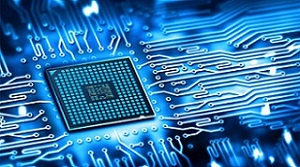
\includegraphics{chip.JPG}
\end{center}
Esta figura muestra un ejemplo de una imagen insertada con el comando includegraphics.
\hfill \break
\begin{figure}[htbp]
  \centering
  \subfigure[Ejemplo 1]{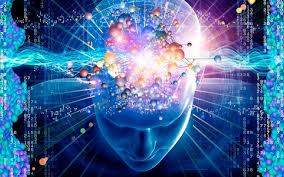
\includegraphics[width=40mm]{ciencia1.JPG}}
  \subfigure[Ejemplo 2]{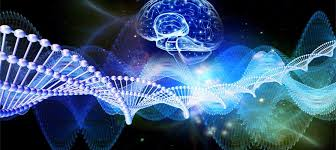
\includegraphics[width=40mm]{ciencia2.JPG}}
  \subfigure[Ejemplo 3]{
\includegraphics[width=80mm]{ciencia3.JPG}}
\end{figure}
Estas tres imágenes muestran un ejemplo de subfiguras insertadas con el comando subfigure, utilizando el parámetro opcional de width, donde se establecen 40mm, 40mm y 80mm de ancho respectivamente.
\hfill \break





%*************************** Manejo de Figuras al lado de tablas (minipage) *****************************/
\section{Manejo de Figuras (Minipage)}
El entorno minipage es utilizado en Latex para cuando se requiera poner dos figuras una al lado de la otra. El nombre minipage se refiere a que se crea una caja que actúa como minicaja, es una miniversión que se inserta dentro de una página. Los comandos necesarios para crear un entorno de minipage se muestra con el siguiente ejemplo.

\begin{verbatim}
  \begin{minipage}}[pos1][long2][pos2]{long1}
    texto
  \end{minipage}
\end{verbatim}

La siguiente tabla explica cada uno de los parámetros del comando minipage.
\begin{center}
  \begin{tabular}[t]{|c|m{5cm}|}
    \hline
    long1 & Este es el único parámetro obligatorio, es el que indica el ancho. \\ \hline
    pos1 & Este parámetro determina la alineación de la caja con respecto al contexto al que se encuentra. \\ \hline
    long2 & Este parámetro determina la altura de la caja. \\ \hline
    pos2 & Este parámetro determina donde se va a colocar el texto dentro de la caja. \\ \hline
  \end{tabular}
\end{center}
\hfill \break

\begin{minipage}[t]{0.2\textwidth}

\includegraphics[width=\textwidth]{ciencia4.JPG}
\end{minipage}
\begin{minipage}[t]{0.2\textwidth}

\includegraphics[width=\textwidth]{ciencia5.JPG}
\end{minipage}

Las imágenes anteriores muestran un ejemplo de minipage, donde se puede visualizar una imagen junto a la otra, ambas dentro de una caja.
\hfill \break





%***************************** Manejo de Ecuaciones Matemáticas ***********************************/
\section{ Ecuaciones Matemáticas }
Una de las principales razones por las cuales \LaTeX\xspace tiene tanta flexibilidad a la hora de crear archivos PDFs, es por el manejo de las ecuaciones matemáticas, de otras maneras puede ser complicado tratar de crear un PDF con tantos símbolos matemáticos.

\begin{itemize}
  \item \textbf{\textit{Ecuaciones: }} Se pueden insertar ecuaciones utilizando un signo de dólar \$. Se puede utilizar para insertar símbolos matemáticos en una oración, por ejemplo $1+2=3$.
Si se desea se pueden utilizar dos signos de dólar \$\$ para mostrar una ecuación en una línea propia. Por ejemplo $$1+2=3$$
Del mismo modo se pueden enumerar las ecuaciones para tener alguna referencia, para eso se deben incluir los siguientes comandos, se muestra un ejemplo del resultado con la numeración de cuatro ecuaciones.
  \begin{center}
    \begin{verbatim}
      \begin{equation} 
        Ecuación ...
      \end{equation}
    \end{verbatim}
  \end{center}
  \begin{equation}
    1+2=3
  \end{equation}
  \begin{equation}
    5-1=4
  \end{equation}
  \begin{equation}
    3*3=9
  \end{equation}
  \begin{equation}
    12/4=3
  \end{equation}

  \LaTeX\xspace también permite tener una ecuación matemática con todos sus pasos en una línea por cada paso. A continuación se muestra cual es el comando necesario para lograrlo y un ejemplo de como se ve implementado en el archivo PDF. Se puede incluir el * para indicarle al comando eqnarray que no es necesario que enumere la ecuación, el comando para esto es el siguiente.
  \begin{center}
    \begin{verbatim}
      \begin{equation*} 
        Ecuación ...
      \end{equation*}
    \end{verbatim}
  \end{center}
  \begin{eqnarray*}
    a & = & b + c \\
    & = & y - z
  \end{eqnarray*}
\end{itemize} % Fin de item Ecuaciones

\begin{itemize}
  \item \textbf{\textit{Símbolos: }} Cuando se requiera insertar símbolos conocidos como +, -, =, !, /, (), [], : y demás, es necesario utilizar un comando. A continuación se muestran una serie de secciones las cuales muestran como hacer inserciones de 'potencias e índices', 'fracciones', 'raíces', 'sumatorias e integrales' y 'letras griegas'.

\subsection{Potencias}
Las potencias se insertan utilizando el símbolo \^{}. Ejemplos pueden ser: $n^5$, $y^2$, $x^3$.

\subsection{Índices}
Los índices se insertan utilizando el símbolo \_. Ejemplos pueden ser $4_i$, $3_y$, $5_p$. En caso de que los índices requieran más de un caracter, se pueden encerrar entre \{\}, por ejemplo $b_{a-8}$.

\subsection{Fracciones}
Las fracciones se insertan utilizando el comando:
  \begin{center}
    \begin{verbatim}
      $$\frac{numerador}{denominador}$$ 
    \end{verbatim}
  \end{center}
Ejemplos de fracciones pueden ser los siguientes: $$\frac{a-b}{6}$$ 

\subsection{Raíces}
Las raíces se insertan utilizando el comando \textbackslash{}sqrt\{...\} donde ... se reemplaza por el contenido de la raíz que se quiera insertar. Se pueden utilizar los paréntesis cuadrados [] para incluir la magnitud de la raíz. Se muestran los comandos con ejemplos respectivos.
  \begin{center}
    \begin{verbatim}
      $$\sqrt{y^4} $$
      $$\sqrt[x]{y^4} $$
      $$\sqrt[x]{(a-b)^4}$$ 
      $$\sqrt[x]{(a-b)^2-i}$$
      $$\sqrt[x]{(t-2)^3-u}$$
    \end{verbatim}
  \end{center}
Ejemplos de los comandos son los siguientes.
      $$\sqrt{y^4}$$ 
      $$\sqrt[x]{y^4}$$ 
      $$\sqrt[x]{(a-b)^4}$$ 
      $$\sqrt[x]{(a-b)^2-i}$$ 
      $$\sqrt[x]{(t-2)^3-u}$$ 

\subsection{Sumatorias}
Para insertar el símbolo de una sumatoria en \LaTeX\xspace se tiene que utilizar el comando \textbackslash{}sum, el límite superior de la sumatoria se indica con el sombrero \^{} y el límite inferior se indica con \_. Los siguientes comandos muestran como insertar una sumatoria.
  \begin{center}
    \begin{verbatim}
      $$\sum_{p=3}^7 t^x$$
      $$\sum_{b=0}^2 p^x-1$$
    \end{verbatim}
  \end{center}
El resultado de dichos comandos son los siguientes respectivamente:
  \begin{center}
     $$\sum_{p=3}^7 t^x$$
     $$\sum_{b=0}^2 p^x-1$$
  \end{center}

\subsection{Integrales}
Para insertar el símbolo de una integral en \LaTeX\xspace se tiene que utilizar el comando \textbackslash{}int, el límite superior de la integral se indica con el sombrero \^{} y el límite inferior se indica con \_. El siguiente comando muestra como insertar una integral.
  \begin{center}
    \begin{verbatim}
      $$\int_y^x f(x)$$
    \end{verbatim}
  \end{center}
El resultado de dicho comando es el siguiente:
$$\int_y^x f(x)$$

\subsection{Letras Griegas}
\LaTeX\xspace también permite la inserción de letras griegas, las cuales se insertan utilizando el nombre de la letra anteponiendo un 'backslash'. Ejemplos de como aplicar dichas letras se pueden ver a continuación.
   \begin{verbatim}
      $\alpha$
      $\beta$
      $\delta, \Delta$
      $\theta, \Theta$
      $\mu$
      $\pi, \Pi$
      $\sigma, \Sigma$
      $\phi, \Phi$
      $\psi, \Psi$
      $\omega, \Omega$
   \end{verbatim}
Los resultados de los comandos anteriores para inserciones de letras griegas se muestran a continuación. \\
\\
      $\alpha$
      $\beta$
      $\delta, \Delta$
      $\theta, \Theta$
      $\mu$
      $\pi, \Pi$
      $\sigma, \Sigma$
      $\phi, \Phi$
      $\psi, \Psi$
      $\omega, \Omega$
\end{itemize}
\hfill \break






%***************************** Manejo de Colores ***********************************/
\section{ Manejo de Colores }
Para el manejo de colores en \LaTeX\xspace, se debe importar el paquete color, a la vez existen dos comandos principales para dicho propósito.
\begin{itemize}
  \item \textbf{\textit{textcolor\{NombreColor\}\{Texto\} }}
\end{itemize}
\begin{itemize}
  \item \textbf{\textit{color\{NombreColor\} }}
\end{itemize}

\subsection{Cambiar color de fuentes }
Para utilizar la paleta básica de colores con el comando textcolor se requiere indicar entre \{\} el color que se requiere y posteriormente también entre \{\} el texto que se quiere visualizar con dicho color especificado, a continuación se muestran los comandos para ejemplos de textos utilizando paletas de colores azul, rojo, verde, amarillo, negro y cyan.
\begin{center}
  \begin{verbatim}
    \textcolor{blue}{texto}
    \textcolor{red}{texto}
    \textcolor{green}{texto}
    \textcolor{yellow}{texto}
    \textcolor{black}{texto}
    \textcolor{cyan}{texto}
  \end{verbatim}
\end{center}
El resultado de implementar dichos colores es el siguiente:
\begin{center}
   \textcolor{blue}{Esto es un texto utilizando color azul!} \\
   \textcolor{red}{Esto es un texto utilizando color rojo!} \\
   \textcolor{green}{Esto es un texto utilizando color verde!} \\
   \textcolor{yellow}{Esto es un texto utilizando color amarillo!} \\
   \textcolor{black}{Esto es un texto utilizando color negro!} \\
   \textcolor{cyan}{Esto es un texto utilizando color cyan!} \\
\end{center}

% Modelos de colores
\subsection{Modelos de colores}
Se pueden utilizar los siguientes tres modelos cuando se requiera personalizar los colores requeridos para los textos.
\begin{itemize}
  \item \textbf{\textit{ rgb (Red Green Blue): }} este modelo utiliza como colores primarios el rojo, verde y azul, para identificar el color requerido utilizando este modelo se deben especificar tres números comprendidos entre el 0 y 1.
\end{itemize}
\begin{itemize}
  \item \textbf{\textit{ cmyk (Cyan Magenta Yellow Black): }} este modelo requiere que se especifiquen cuatro números comprendidos entre 0 y 1, especificando para cada uno de los colores del cmyk la combinación requerida. Este método es conocido por ser el utilizado en las impresoras.
\end{itemize}
\begin{itemize}
  \item \textbf{\textit{ gray: }} este modelo utiliza una escala de grises, indicando un número único comprendido entre 0 y 1.
\end{itemize}

\hfill \break
Se pueden hacer combinaciones de colores utilizando los modelos anteriormente mencionados, a continuación se muestran los comandos necesarios para poder hacer uso de los modelos.
\begin{center}
  \begin{verbatim}
    \textcolor[rgb]{1,0,0}{Rojo}
    \textcolor[rgb]{1,1,0}{Amarillo}
    \textcolor[rgb]{0.2,0.5,0.7}{Azulado}
    \textcolor[cmyk]{0,1,0,0}{Magenta}
    \textcolor[cmyk]{1,0,1,0}{Verde}
    \textcolor[gray]{0.3}{Gris Oscuro}
    \textcolor[gray]{0.7}{Gris Claro}
  \end{verbatim}
\end{center}
El resultado de implementar dichos colores es el siguiente:
\begin{center}
    \textcolor[rgb]{1,0,0}{Rojo}\\
    \textcolor[rgb]{1,1,0}{Amarillo}\\
    \textcolor[rgb]{0.2,0.5,0.7}{Azulado}\\
    \textcolor[cmyk]{0,1,0,0}{Magenta}\\
    \textcolor[cmyk]{1,0,1,0}{Verde}\\
    \textcolor[gray]{0.3}{Gris Oscuro}\\
    \textcolor[gray]{0.7}{Gris Claro}
\end{center}

% Cajas de color
\subsection{Cajas de color}
\LaTeX\xspace permite no solo colorear textos, sino que también se pueden realizar cajas con colores de fondo, esta sección muestra los comandos necesarios para implementar cajas coloreadas en un PDF compilado con \LaTeX\xspace.
\begin{verbatim}
\colorbox[rgb]{0.5,0.5,1}{caja roja y azul 50\%}
\colorbox{yellow}{caja de color amarilla}
\colorbox{cyan}{caja de color cyan}
\colorbox{green}{caja de color verde}
\end{verbatim}
El resultado de implementar dichos colores es el siguiente:
\begin{center}
  \colorbox[rgb]{0.5,0.5,1}{caja roja y azul 50\%}
  \colorbox{yellow}{caja de color amarilla}
  \colorbox{cyan}{caja de color cyan}
  \colorbox{green}{caja de color verde}
\end{center}

% Bordes de color
\subsection{Bordes de color}
\LaTeX\xspace también permite crear bordes con distintos colores para una caja, esta sección muestra los comandos necesarios para implementar cajas coloreadas con un borde de color. A la vez es posible especificar un grosor para el borde a colorear utilizando el comando \textbackslash{}setlength\{fboxrule\}\{3 pt\}.
\begin{verbatim}
\colorbox[rgb]{0.5,0.5,1}{caja roja y azul 50\%}
\fcolorbox{red}{yellow}{caja amarilla y borde rojo}
\setlength{\fboxrule}{3 pt}
\fcolorbox{red}{cyan}{caja cyan y borde rojo}
\setlength{\fboxrule}{3 pt}
\fcolorbox{red}{green}{caja verde y borde rojo}
\fcolorbox{green}{yellow}{caja amarilla y borde verde}
\end{verbatim}
El resultado de implementar dichos colores de bordes en las cajas es el siguiente:
\begin{center}
    \colorbox[rgb]{0.5,0.5,1}{caja roja y azul 50\%}\\
    \fcolorbox{red}{yellow}{caja amarilla y borde rojo}\\
    \setlength{\fboxrule}{3 pt}
    \fcolorbox{red}{cyan}{caja cyan y borde rojo}\\
    \setlength{\fboxrule}{3 pt}
    \fcolorbox{red}{green}{caja verde y borde rojo} \\
    \fcolorbox{green}{yellow}{caja amarilla y borde verde}
\end{center}

\hfill \break
\hfill \break
\hfill \break





%\section{Conclusion}
%The conclusion goes here.





% if have a single appendix:
%\appendix[Proof of the Zonklar Equations]
% or
%\appendix  % for no appendix heading
% do not use \section anymore after \appendix, only \section*
% is possibly needed

% use appendices with more than one appendix
% then use \section to start each appendix
% you must declare a \section before using any
% \subsection or using \label (\appendices by itself
% starts a section numbered zero.)
%


%\appendices
%\section{Proof of the First Zonklar Equation}
%Appendix one text goes here.

% you can choose not to have a title for an appendix
% if you want by leaving the argument blank
%\section{}
%Appendix two text goes here.


% use section* for acknowledgment
%\section*{Acknowledgment}


%The authors would like to thank...


% Can use something like this to put references on a page
% by themselves when using endfloat and the captionsoff option.
\ifCLASSOPTIONcaptionsoff
  \newpage
\fi



% trigger a \newpage just before the given reference
% number - used to balance the columns on the last page
% adjust value as needed - may need to be readjusted if
% the document is modified later
%\IEEEtriggeratref{8}
% The "triggered" command can be changed if desired:
%\IEEEtriggercmd{\enlargethispage{-5in}}

% references section

% can use a bibliography generated by BibTeX as a .bbl file
% BibTeX documentation can be easily obtained at:
% http://mirror.ctan.org/biblio/bibtex/contrib/doc/
% The IEEEtran BibTeX style support page is at:
% http://www.michaelshell.org/tex/ieeetran/bibtex/
\bibliographystyle{IEEEtran}
% argument is your BibTeX string definitions and bibliography database(s)
\bibliography{bibliography}



% that's all folks
\end{document}


